\section{Test Cases}
The following test cases were executed.
\subsection{Encoder - Test XML Response}
\begin{flushleft}
This test case checks the generated XML file from the encoder module. 
The generated XML’s structure and values are checked against the expected XML.

\vspace*{1em}

\begin{figure}[h!]
    \centering
    \frame{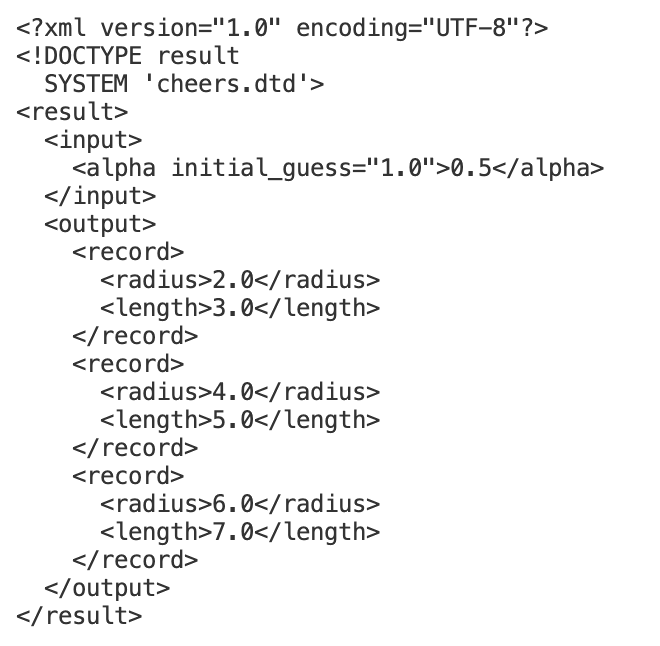
\includegraphics[scale= 0.4]{resources/expected/expected_xml.png}}
    \caption{Expected XML}
    \label{fig:XML output}
  \end{figure}

\vspace*{1em}

\begin{tabular}{ |p{6cm}||p{6cm} |  }
    \hline
    \multicolumn{2}{|c|}{\textbf{Encoder - Test XML Response}} \\
    \hline
    \textbf{Input} & \textbf{Expected Output}\\
    \hline
    \textit{initial\_guess} = 1.0   & \multirow{3}{15em}{The encoder must generate an XML conforming to the DTD, with values matching the expected values.} \\
    \textit{alpha} = 0.5 &   \\
    \textit{records} = [(2.0, 3.0), (4.0, 5.0), (6.0, 7.0)] & \\
    
    \hline
\end{tabular}
\end{flushleft}


\vspace*{1em}
\subsection{Encoder - Test CSV Response}
\begin{flushleft}
    This test case checks the generated csv file from the encoder module. 
    For every line in the CSV, the calculated value is checked against the expected value.
\vspace*{1em}

\begin{figure}[h!]
    \centering
    \frame{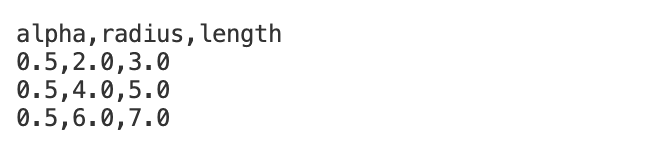
\includegraphics[scale= 0.4]{resources/expected/expected_csv.png}}
    \caption{Expected CSV}
    \label{fig:CSV output}
  \end{figure}
\vspace*{1em}

\begin{tabular}{ |p{6cm}||p{6cm} |  }
    \hline
    \multicolumn{2}{|c|}{\textbf{Encoder - Test CSV Response}} \\
    \hline
    \textbf{Input} & \textbf{Expected Output}\\
    \hline
    \textit{alpha} = 0.5 & \multirow{3}{15em}{The encoder must generate a CSV file matching the expected values.} \\
    \textit{records} = [(2.0, 3.0), (4.0, 5.0), (6.0, 7.0)] & \\
    
    \hline
\end{tabular}
\end{flushleft}

\vspace*{1em}
\subsection{Math - Test Sin}
\begin{flushleft}
    This test case checks the sin() function in the Math and libmath library/module. 
    The Sin values returned from the Math library and libmath module have been compared.
\vspace*{1em}

\begin{tabular}{ |p{6cm}||p{6cm} |  }
    \hline
    \multicolumn{2}{|c|}{\textbf{Math - Test Sin}} \\
    \hline
    \textbf{Input} & \textbf{Expected Output}\\
    \hline
    \textit{libmath.sin(0), math.sin (0)}   & Calculated values must be almost equal \\
    \hline
    \textit{libmath.sin(math.pi), math.sin(math.pi)} & Calculated values must be almost equal \\
    \hline
    \textit{libmath.sin(math.pi/2), math.sin(math.pi/2)}  & Calculated values must be almost equal \\
    \hline
\end{tabular}
\end{flushleft}

\vspace*{1em}
\subsection{Math - Test Cos}
\begin{flushleft}
    This test case checks the cos() function in the Math and libmath library/module.
    The Cos values returned from the Math library and libmath module have been compared. 
\vspace*{1em}

\begin{tabular}{ |p{6cm}||p{6cm} |  }
    \hline
    \multicolumn{2}{|c|}{\textbf{Math - Test Cos}} \\
    \hline
    \textbf{Input} & \textbf{Expected Output}\\
    \hline
    \textit{libmath.cos(0), math.cos(0)}   & Calculated values must be almost equal \\
    \hline
    \textit{libmath.cos(math.pi), math.cos(math.pi)} & Calculated values must be almost equal \\
    \hline
    \textit{libmath.cos(math.pi/2), math.cos(math.pi/2)}  & Calculated values must be almost equal \\
    \hline
\end{tabular}
\end{flushleft}

\subsection{Math - Test Pi}
\vspace*{1em}
\begin{flushleft}
    This test case checks the pi value in the Math library and the value\_of\_pi() method in the libmath module. 
    The Pi value has been approximated 1000 times in the value\_of\_pi() method. 
    The Pi values returned from the Math library and libmath module have been compared.
\vspace*{1em}

\begin{tabular}{ |p{6cm}||p{6cm} |  }
    \hline
    \multicolumn{2}{|c|}{\textbf{Math - Test Pi}} \\
    \hline
    \textbf{Input} & \textbf{Expected Output}\\
    \hline
    \textit{libmath.value\_of\_pi(1000),math.pi, places = 2}   & Calculated values must be almost equal \\
    \hline
\end{tabular}
\end{flushleft}

\vspace*{1em}
\subsection{Math - Test Factorial}
\begin{flushleft}
    This test case checks the factorial calculated by the libmath module. 
    The calculated value is compared against the a few expected values.
\vspace*{1em}

\begin{tabular}{ |p{6cm}||p{6cm} |  }
    \hline
    \multicolumn{2}{|c|}{\textbf{Math - Test Factorial}} \\
    \hline
    \textbf{Input} & \textbf{Expected Output}\\
    \hline
    \textit{libmath.factorial(0)}, 1   & Calculated and expected value must match \\
    \hline
    \textit{libmath.factorial(1)}, 1  & Calculated and expected value must match \\
    \hline
    \textit{libmath.factorial(5)}, 120   & Calculated and expected value must match \\
    \hline
\end{tabular}
\end{flushleft}

\vspace*{1em}

\subsection{Root Approximation - Test Numeric}
\begin{flushleft}
    This test case checks if an exception is thrown when a non-numeric epsilon (accuracy) value is passed to the newton\_method() function.
\vspace*{1em}

\begin{tabular}{ |p{6cm}||p{6cm} |  }
    \hline
    \multicolumn{2}{|c|}{\textbf{Root Approximation - Test Numeric}} \\
    \hline
    \textbf{Input} & \textbf{Expected Output}\\
    \hline
    \textit{newton\_method(callable(), callable(), 'a')}   & A 'Value Error' exception must be raised. \\
    \hline
\end{tabular}
\end{flushleft}

\vspace*{1em}

\subsection{Root Approximation - Test Positive}
\begin{flushleft}
    This test case checks if an exception is thrown when a negative epsilon (accuracy) value is passed to the newton\_method() function.
\vspace*{1em}

\begin{tabular}{ |p{6cm}||p{6cm} |  }
    \hline
    \multicolumn{2}{|c|}{\textbf{Root Approximation - Test Positive}} \\
    \hline
    \textbf{Input} & \textbf{Expected Output}\\
    \hline
    \textit{newton\_method(callable(), callable(), '-0.01')}   & A 'Value Error' exception must be raised. \\
    \hline
\end{tabular}
\end{flushleft}

\vspace*{1em}

\subsection{Root Approximation - Test Divide by Zero}
\begin{flushleft}
    This test case checks the callable lambda function passed to newton\_method() function. 
\vspace*{1em}

\begin{tabular}{ |p{6cm}||p{6cm} |  }
    \hline
    \multicolumn{2}{|c|}{\textbf{Root Approximation - Test Divide by Zero}} \\
    \hline
    \textbf{Input} & \textbf{Expected Output}\\
    \hline
    \textit{newton\_method(callable(), lambda x: 0, 1)}   & None must be returned. \\
    \hline
\end{tabular}
\end{flushleft}

\vspace*{1em}
\subsection{Root Approximation - Error Tolerance}
\begin{flushleft}
    This test case checks if the error tolerance in the value calculated by newton\_method() is less than 0.0001. 
    Value for Sin, Pi and Cos have been obtained from the libmath module.
 
\vspace*{1em}

\begin{tabular}{ |p{6cm}||p{6cm} |  }
    \hline
    \multicolumn{2}{|c|}{\textbf{Root Approximation - Error Tolerance}} \\
    \hline
    \textbf{Input} & \textbf{Expected Output}\\
    \hline
    \textit{newton\_method(lambda a: a - sin(a) - PI/2, lambda a: 1 - cos(a), 1)}   & Calculated Value - 2.309878472457841 < 0.0001 \\
    \hline
\end{tabular}
\end{flushleft}
\vspace*{1em}

\subsection{Execution Results}

All the test cases passed the test and the code coverage reached 100\%.

\begin{figure}[h!]
    \centering
    \frame{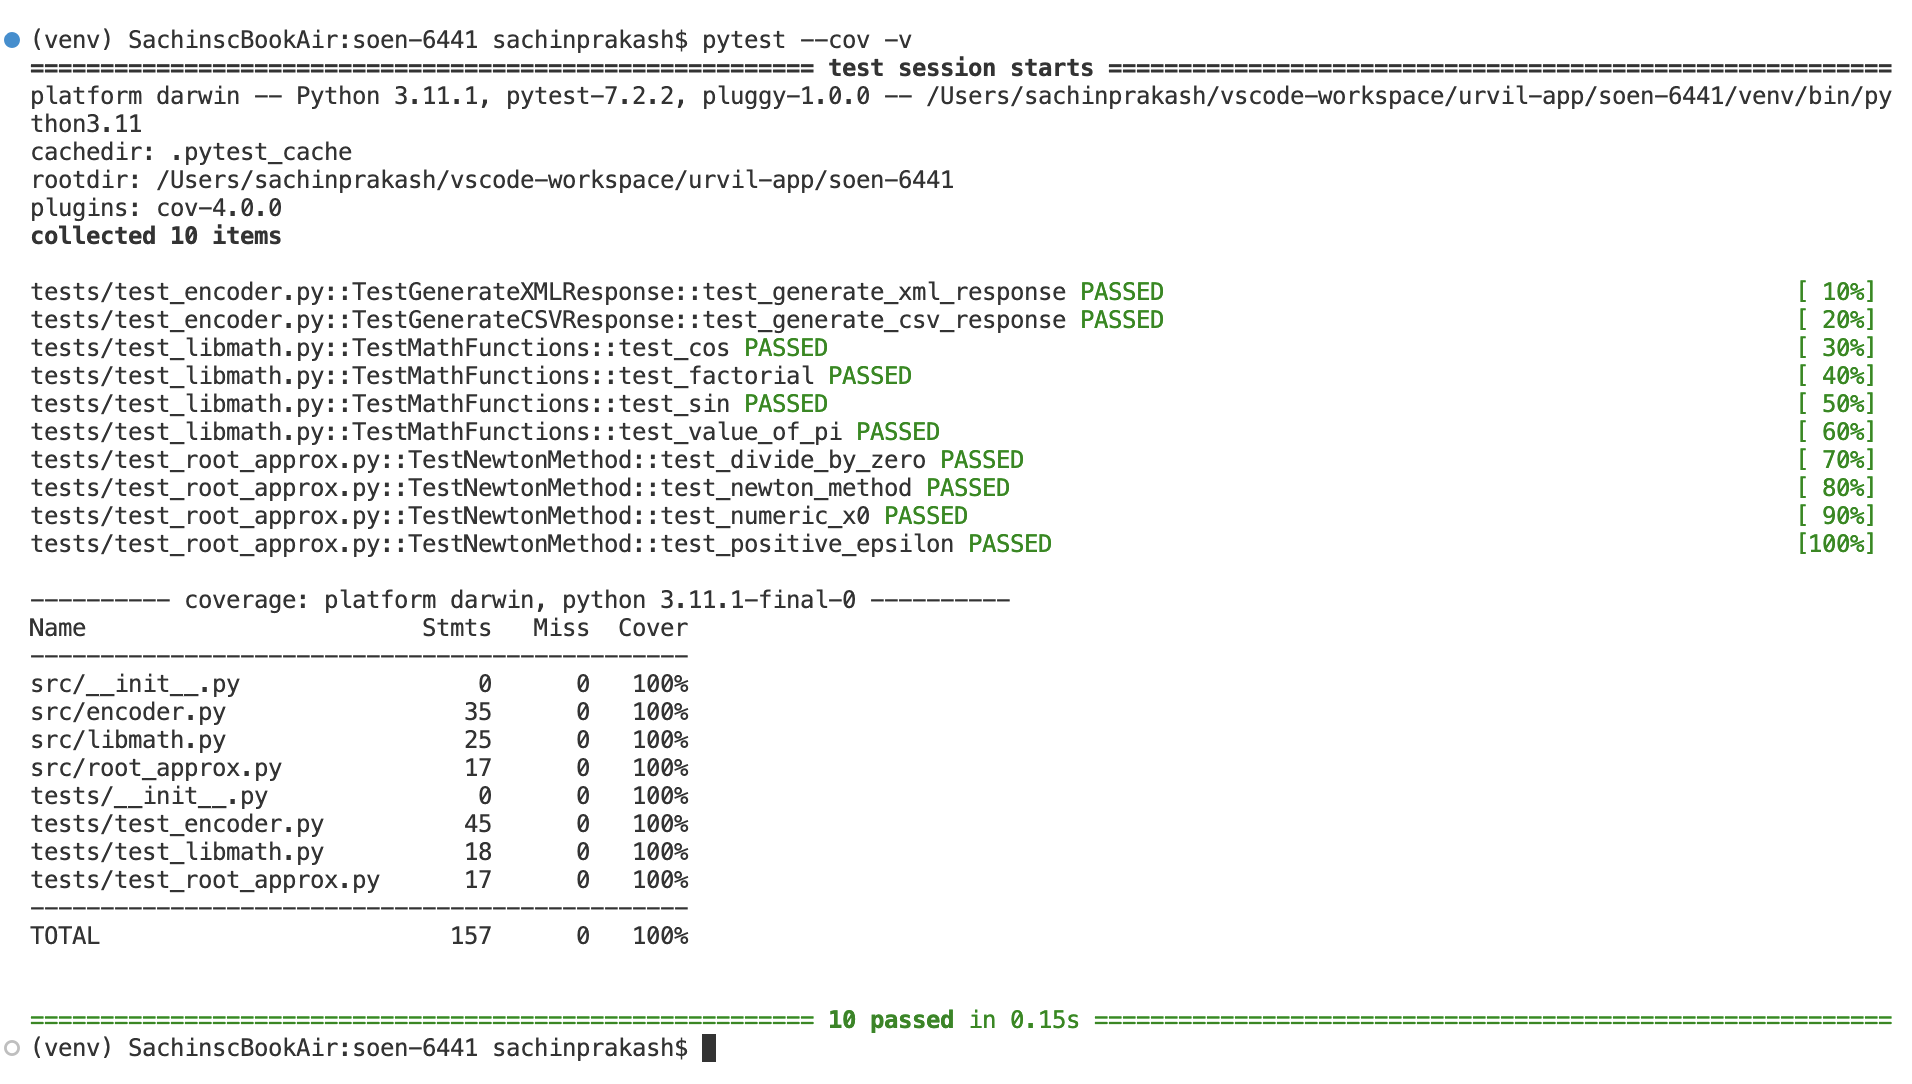
\includegraphics[scale= 0.4]{resources/tc_ex_results.png}}
    \caption{Test Results}
    \label{fig:Results and Coverage}
\end{figure}